% The contents of this file is 
% Copyright (c) 2009-  Charles R. Severance, All Righs Reserved
\chapter{?`Por qu\'e se debe aprender a programar?}

Escribir programas (o programar) es una actividad muy creativa gratificante. Usted puede escribir programas para ganarse la vida o para resolver un problema de an\'alisis dif\'icil o simplemente por el placer de poder ayudar a alguien a resolver un problema. Este libro asume que \textbf{todos} necesitan saber cómo programar y que una vez que se aprende se descubre lo que se quiere lograr con la nueva destreza adquirida.  

Estamos rodeados en nuestra vida diaria de computadoras que van desde p\'ortatiles a tel\'efonos celulares. Se puede pensar de estas computadoras como si fueran nuestros ``asistentes personales'', quienes realizan muchas de las tareas en nuestro lugar. El \textit{hardware} en las computadoras de hoy est\'an construidas esencialmente para que continuamente hagan la pregunta, 
``?`Qu\'e quieres que haga despu\'es?''.

\beforefig
\centerline{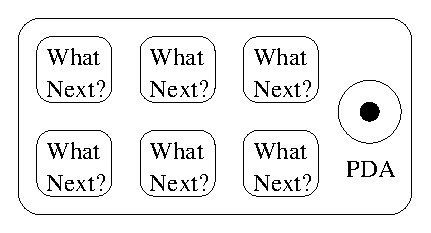
\includegraphics[height=1.00in]{figs2/pda.eps}}
\afterfig

Los programadores agreagan un sistema operativo y una serie de aplicaciones al \textit{hardware} y nosotros terminamos con un Asistente Personal Digital muy \'util para diferentes cosas.

Nuestras computadoras son r\'apidas y tienen una vasta cantidad de memoria y podr\'ian ser muy \'utiles si tan solo supi\'eramos el lenguage para hablarles y explicarles lo que quisi\'eramos que ``hagan despu\'es''. Si supi\'eramos este lenguage podr\iamos decirle a la computadora que haga tareas repetitivas a nombre nuestro. Interesantemente, el tipo de cosas que las computadoras hacen mejor, a menudo, son cosas que los humanos encontramos aburridas y abrumadoras.

Por ejemplo, mire los tres primeros p\'arrafos de este cap\'itulo y d\'igame cu\'al es la palabra m\'as com\'un. Mientras que usted es capaz de leer y comprender las palabras en cuesti\'on de segundos, contarlas es doloroso porque no es el tipo de problema que la mente humana ha sido dise\~nada para resolver. Para una computadora es todo lo contrario, leer y comprender el texto de un pedazo de papel es dif\'icil para una computadora, pero contar las palabras y decirle a usted cu\'antas veces la palabra m\'as com\'un fue usada es muy f\'acil para la computadora:

\beforeverb
\begin{verbatim}
python palabras.py
Enter file:palabras.txt
de 7
\end{verbatim}
\afterverb
%
Nuestro ``asistente personal de an\'alisis de informaci\'on'' nos dice r\'apidamente que la palabra ``de'' aparece 7 veces en los primeros tres p\'arrafos de este cap\'itulo.

El hecho de que las computadoras sean tan buenas en lo que los humanos no lo son es la raz\'on por la cual usted debe desarrollar la destreza de hablar el ``lenguage de computadora''. Una vez que aprenda este lenguage ver\'a c\'omo puede delegar tareas miniales a su socia (la computadora), liberando as\'i su tiempo para hacer aquellas cosas para las que ha sido creado de manera especial. Usted aporta creatividad, intuici\'on e inventividad a esta relaci\'on colaborativa.  

\section{Creatividad y motivaci\'on}

Aunque este libro no est\'a dirigido a programadores profesionales, la prgramaci\'on puede ser un trabajo muy gratificante tanto personal como financieramente. 
Elaborar programas \'utiles, elegantes e inteligentes para el beneficio de otros es una actividad muy creativa. Su computadora o Asistente Personal Digital (PDA por sus siglas en ingl\'es) 
generalmente contine diferentes programas de diferentes programadores, cada uno de ellos compitiendo por su atenci\'on e inter\'es. Ellos tratan de hacer lo mejor para satisfacer sus necesidades y proveerle una excelente experiencia de usuario en el proceso. En algunas situaciones, cuando usted escoge una aplicaci\'on (software), los programadores son directamente compensado en virtud de su elecci\'on.

Al considerar los programas como obras creativas de grupos de programadores, quiz\'a la siguiente imagen sea una versi\'on m\'as sensible de nuestro PDA:

\beforefig
\centerline{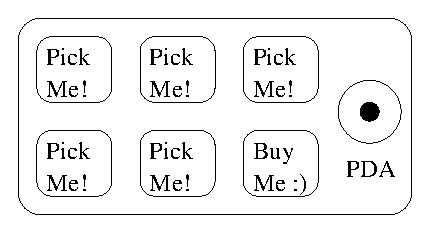
\includegraphics[height=1.00in]{figs2/pda2.eps}}
\afterfig

Por ahora, nuestra motivaci\'on primordial no es hacer dinero o complacer a los usuarios, sino hacernos m\'as productivos en el manejo de datos e informaci\'on que encontraremos en nuestra vida diaria.
Cuando usted comience, usted es tanto programador como usuario de sus propios programas. En la medida en que adquiera m\'as destreza como programador y programar se sienta como una actividad m\'as y m\'as creativa para usted, se le ocurrir\'an ideas sobre el desarrollo de programas para otros.

\section{Arquitectura del hardware de la computadora}
\index{hardware}
\index{hardware!arquitectura}

Antes de comenzar a aprender el lenguage necesario para darle instrucciones a las computadoras para desarrollar software, es necesario aprender una peque\~na cantidad sobre c\'omo se construyen las computadoras. Si usted desbaratara su computadoras o tel\'efono celular y mirara lo que hay dentro, encontar\'ia las siguientes partes:

\beforefig
\centerline{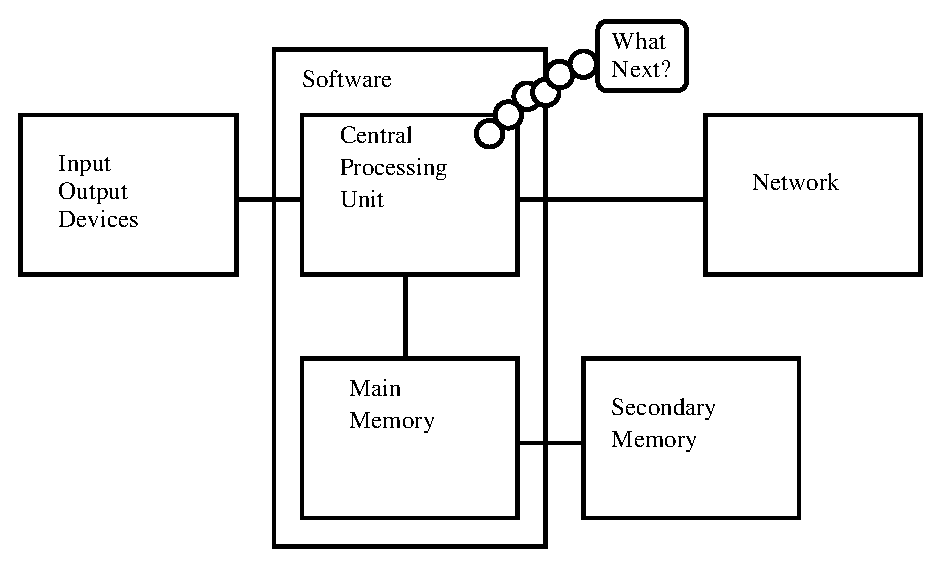
\includegraphics[height=2.50in]{figs2/arch.eps}}
\afterfig

Las definiciones funcionales de alto nivel de estas partes son las siguientes:

\begin{itemize}

\item La {\bf Unidad Central de Procesamiento} conocida por sus siglas en ingl\'es como CPU es esa parte de la computadora que ha sido construida para obsesionarse con la cuesti\'on ``?`qu\'e hay que hacer despu\'es?''. Si su computadora tiene una capacidad de 3.0 Gigahertz, eso significa que el CPU preguntar\'a ``?`qu\'e hay que hacer despu\'es?''
tres mil millones de veces por segundo. Usted va a tener que aprender c\'omo hablar r\'apido para mantener el ritmo de la CPU.

\item The {\bf Memoria Principal} se usa para almacenar la informaci\'on
que la CPU necesita de af\'an. La memoria principal es casi tan r\'apida como la CPU, pero la informaci\'on almacenada en la memoria principal desaparece cuando se apaga la computadora.

\item La {\bf Memoria Secundaria} tambi\'en se usa para almacenar informaci\'on, pero es mucho m\'as lenta que memoria principal.
La ventaja de la memoria secundaria es que puede almacenar informaci\'on aun cuando la computadora est\'e apagada. Ejemplos de la memoria secundaria son los discos duros o memorias flash (esto se encuentran t\'ipicamente en dispositivos USB y reproductores de m\'usica portables).

\item The {\bf Dispositivos de entrada y salida (Input y Output)} son su monitor, teclado, mouse, microf\'ono, parlantes, tablero t\'actil integrado, etc.  
Estos representan todas las formas en que interactuamos con la computadora.

\item Hoy en d\'ia la mayor\'ia de las computadoras tambi\'en tienen
{\bf Conecci\'on a la Red (Network Connection)} para recibir informaci\'oon por medio de una red.
Se puede pensar de una red como un lugar muy lento para almacenar y recuperar datos que pordr\'ian no estar siempre ``actualizados''. En cierto sentido, la red es m\'as lenta y a veces una forma poco fiable de
{\bf Memoria Secundaria}

\end{itemize}

Mientras que la mayor\'ia de los detalles sobre c\'omo trabajan estos componentes es mejor dej\'arselo a los  que construyen computadoras, conocer la terminolog\'ia ayuda para podernos referir a estos componentes cuando escribimos nuestros programas.

Como programador, su trabajo es utilizar y coordinar cada uno de estos recursos para dar soluci\'on a lo problemas para los cuales usted necesita an\'alizar los datos que necesita usar. Como programador usted va a ``hablarle'' la mayor\'ia del tiempo a la CPU para decirle ``qu\'e debe hacer despu\'es''. Algunas veces usted le va a decir a la CPU que utilice memoria principal, la memoria secundaria, la red o los dispositivos de entrada/salida (input/output).

\beforefig
\centerline{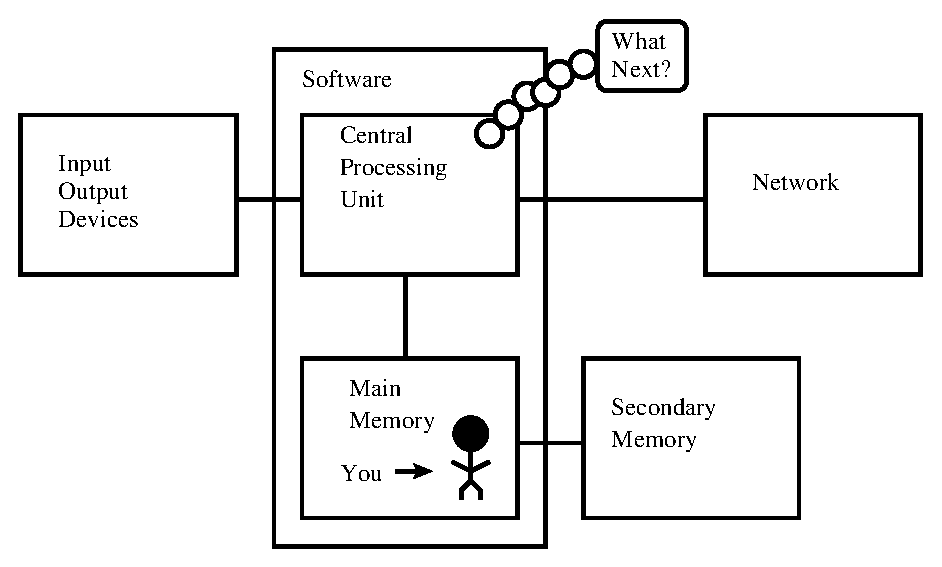
\includegraphics[height=2.50in]{figs2/arch2.eps}}
\afterfig

Usted tiene que ser la persona que le responda a la CPU la pregunta ``?`Qu\'e despu\'es?'', pero ser\'ia muy inc\'omodo reducirlo a usted a un tama\~no de 5mm e insertarlo en la computadora solo para poder emitir un comando tres mil millones de veces por segundo. As\'i que en vez de hacer eso, usted debe escribir sus instrucciones de antemano.
A estas instrucciones almancenadas les llamamos {\bf programa} y al acto de escribir estas instrucciones y escribirlas correctamente {\bf programaci\'on}.

\section{Comprender el concepto de programaci\'on}

En el resto de este libro vamos a tratar de convertirlo a usted en una persona
con destreza en el arte de programaci\'on. Al final, usted ser\'a un 
{\bf programador} --- quiz\'a no un programador profesional, pero por lo menos tendr\'a las destrezas para mirar un problema de an\'alisis de informaci\'on y datos y desarrollar un programa como soluci\'on al problema.

\index{resoluci\'on de problemas}

En un sentido, usted necesita dos destrezas para ser programador:

\begin{itemize}

\item Primero, usted necesita saber el lenguage de programaci\'on (Python) -
usted necesita saber el vocabulario y la gram\'atica. Usted necesita ser capaz de deletrear las palabras en este nuevo lenguage apropiadamente y saber c\'omo construir ``oraciones'' bien formadas en este nuevo lenguage.

\item Segundo, usted necesita ``contar una historia''. Al escribir una historia,
usted combina palabras y oraciones para transmitirle al lector una idea. Componer una historia requiere de destreza y arte, y la destreza de escribir se mejora escribiendo y recibiendo retroalimentaci\'on. En programaci\'on, nuestro programa es la ``historia'' y el problema que usted trata de resolver es la ``idea''.

\end{itemize}

Una vez que usted aprende un programa como Python, encontrar\'a mucho m\'as f\'acil aprender un segundo lenguage de programaci\'on como JavaScript o C++. El nuevo lenguage de programaci\'on tiene un vocabulario y gram\'atica muy diferente, pero una vez que adquiera destreza en la resoluci\'on de problemas, las destrezas van a ser las mismas para todos los lenauages de programaci\'on.

Usted aprender\'a el ``vocabulario'' y ``oraciones'' de Python bien r\'apido.
Le tomar\'a m\'as tiempo aprender a escribir un programa coherente para resolver un problema nuevo. Ense\~namos programaci\'on como ense\~namos escritura. Empezamos leyendo y explicando programas y desp\'es escribimos programas sencillos para luego escribir programas m\'as complejos, en el transcurso del tiempo.
En alg\'un momento usted encuentra ``su inspiraci\'on'' y comienza a descubrir patrones usted mismo y puede ver de manera m\'as natural c\'omo tomar un problema y escribir un programa para darle una soluci\'on, y una vez que llegue a ese punto, la programaci\'on se convierte en un proceso agradable y creativo.  

Comenzamos con el vocabulario y la estructura de los programas de Python. Tenga paciencia cuando la sencillez de los ejemplos le recuerden cuando comenz\'o a leer por primera vez. 

\section{Palabras y oraciones}
\index{lenguage de programaci\'on}
\index{lenguage!programaci\'on}

Unlike human languages, the Python vocabulary is actually pretty small.
We call this ``vocabulary'' the ``reserved words''.  These are words that
have very special meaning to Python.  When Python sees these words in 
a Python program, they have one and only one meaning to Python.  Later
as you write programs you will make your own words that have meaning to 
you called {\bf variables}.   You will have great latitude in choosing
your names for your variables, but you cannot use any of Python's 
reserved words as a name for a variable.

In a sense, when we train a dog, we would use special words like,
``sit'', ``stay'', and ``fetch''.  Also when you talk to a dog and
don't use any of the reserved words, they just look at you with a 
quizzical look on their faces until you say a reserved word.  
For example, if you say, 
``I wish more people would walk to improve their overall health.'', 
what most dogs likely hear is,
``blah blah blah {\bf walk} blah blah blah blah.''
That is because ``walk'' is a reserved word in dog language.  Many
might suggest that the language between humans and cats has no
reserved words\footnote{\url{http://xkcd.com/231/}}.

The reserved words in the language where humans talk to 
Python incudes the following:

\beforeverb
\begin{verbatim}
and       del       from      not       while    
as        elif      global    or        with     
assert    else      if        pass      yield    
break     except    import    print              
class     exec      in        raise              
continue  finally   is        return             
def       for       lambda    try
\end{verbatim}
\afterverb
%
That is it, and unlike a dog, Python is already completely trained.
When you say ``try'', Python will try every time you say it without
fail.

We will learn these reserved words and how they are used in good time,
but for now we will focus on the Python equivalent of ``speak'' (in 
human to dog language).  The nice thing about telling Python to speak
is that we can even tell it what to say by giving it a message in quotes:

\beforeverb
\begin{verbatim}
print 'Hello world!'
\end{verbatim}
\afterverb

And we have even written our first syntactically correct Python sentence.
Our sentence starts with the reserved word {\bf print} followed
by a string of text of our choosing enclosed in single quotes.

\section{Conversaci\'on con Python}

Now that we have a word and a simple sentence that we know in Python,
we need to know how to start a conversation with Python to test 
our new language skills.

Before you can converse with Python, you must first install the Python
software on your computer and learn how to start Python on your 
computer.  That is too much detail for this chapter so I suggest
that you consult \url{www.pythonlearn.com} where I have detailed
instructions and screencasts of setting up and starting Python 
on Macintosh and Windows systems.  At some point, you will be in 
a terminal or command window and you will type {\bf python} and 
the Python interpreter will start executing in interactive mode
and appear somewhat as follows:
\index{interactive mode}

\beforeverb
\begin{verbatim}
Python 2.6.1 (r261:67515, Jun 24 2010, 21:47:49) 
[GCC 4.2.1 (Apple Inc. build 5646)] on darwin
Type "help", "copyright", "credits" or "license" for more information.
>>> 
\end{verbatim}
\afterverb
%
The {\tt >>>} prompt is the Python interpreter's way of asking you, ``What
do you want me to do next?''.  Python is ready to have a conversation with
you.  All you have to know is how to speak the Python language and you 
can have a conversation.

Lets say for example that you did not know even the simplest Python language
words or sentences. You might want to use the standard line that astronauts 
use when they land on a far away planet and try to speak with the inhabitants
of the planet:

\beforeverb
\begin{verbatim}
>>> I come in peace, please take me to your leader
  File "<stdin>", line 1
    I come in peace, please take me to your leader
         ^
SyntaxError: invalid syntax
>>> 
\end{verbatim}
\afterverb
%
This is not going so well.  Unless you think of something quickly,
the inhabitants of the planet are likely to stab you with their spears, 
put you on a spit, roast you over a fire, and eat you for dinner.

Luckily you brought a copy of this book on your travels and you thumb to
this very page and try again:

\beforeverb
\begin{verbatim}
>>> print 'Hello world!'
Hello world!
\end{verbatim}
\afterverb
%
This is looking much better so you try to communicate some
more:

\beforeverb
\begin{verbatim}
>>> print 'You must be the legendary god that comes from the sky'
You must be the legendary god that comes from the sky
>>> print 'We have been waiting for you for a long time'
We have been waiting for you for a long time
>>> print 'Our legend says you will be very tasty with mustard'
Our legend says you will be very tasty with mustard
>>> print 'We will have a feast tonight unless you say
  File "<stdin>", line 1
    print 'We will have a feast tonight unless you say
                                                     ^
SyntaxError: EOL while scanning string literal
>>> 
\end{verbatim}
\afterverb
%
The conversation was going so well for a while and then you
made the tiniest mistake using the Python language and Python 
brought the spears back out.

At this point, you should also realize that while Python 
is amazingly complex and powerful and very picky about 
the syntax you use to communicate with it, Python is {\em 
not} intelligent.  You are having a conversation with 
yourself but using proper syntax.

In a sense when you use a program written by someone else
the conversation is between you and those other
programmers with Python acting as an intermediary.  Python
is a way for the creators of programs to express how the 
conversation is supposed to proceed.  And
in just a few more chapters, you will be one of those
programmers using Python to talk to the users of your program.

Before we leave our first conversation with the Python 
interpreter, you should probably know the proper way
to say ``good-bye'' when interacting with the inhabitants
of Planet Python:

\beforeverb
\begin{verbatim}
>>> good-bye
Traceback (most recent call last):
  File "<stdin>", line 1, in <module>
NameError: name 'good' is not defined

>>> if you don't mind, I need to leave
  File "<stdin>", line 1
    if you don't mind, I need to leave
             ^
SyntaxError: invalid syntax

>>> quit()
\end{verbatim}
\afterverb
%
You will notice that the error is different for the first two
incorrect attempts.   The second error is different because 
{\bf if} is a reserved word and Python saw the reserved word
and thought we were trying to say something but got the syntax
of the sentence wrong.

The proper way to say ``good-bye'' to Python is to enter 
{\bf quit()} at the interactive chevron {\tt >>>} prompt.
It would have probably taken you quite a while to guess that 
one so having a book handy probably will turn out 
to be helpful.

\section{Terminolog\'ia: interprete y compilador}

Python is a {\bf high-level} language intended to be relatively
straightforward for humans to read and write and for computers
to read and process.  Other high-level languages include: Java, C++,
PHP, Ruby, Basic, Perl, JavaScript, and many more.  The actual hardware
inside the Central Processing Unit (CPU) does not understand any
of these high level languages.

The CPU understands a language we call {\bf machine-language}.  Machine
language is very simple and frankly very tiresome to write because it 
is represented all in zeros and ones:

\beforeverb
\begin{verbatim}
01010001110100100101010000001111
11100110000011101010010101101101
...
\end{verbatim}
\afterverb
%
Machine language seems quite simple on the surface given that there 
are only zeros and ones, but its syntax is even more complex
and far more intricate than Python.  So very few programmers ever write
machine language.  Instead we build various translators to allow
programmers to write in high level languages like Python or JavaScript
and these translators convert the programs to machine language for actual
execution by the CPU.

Since machine language is tied to the computer hardware, machine language
is not {\bf portable} across different types of hardware.  Programs written in 
high-level languages can be moved between different computers by using a 
different interpreter on the new machine or re-compiling the code to create
a machine language version of the program for the new machine.

These programming language translators fall into two general categories:
(1) interpreters and (2) compilers.

An {\bf interpreter} reads the source code of the program as written by the
programmer, parses the source code, and interprets the instructions on-the-fly.
Python is an interpreter and when we are running Python interactively, 
we can type a line of Python (a sentence) and Python processes it immediately
and is ready for us to type another line of Python.   

Some of the lines of Python tell Python that you want it to remember some 
value for later.   We need to pick a name for that value to be remembered and
we can use that symbolic name to retrieve the value later.  We use the 
term {\bf variable} to refer to the labels we use to refer to this stored data.

\beforeverb
\begin{verbatim}
>>> x = 6
>>> print x
6
>>> y = x * 7
>>> print y
42
>>> 
\end{verbatim}
\afterverb
%
In this example, we ask Python to remember the value six and use the label {\bf x}
so we can retrieve the value later.   We verify that Python has actually remembered
the value using {\bf print}. Then we ask Python to retrieve {\bf x} and multiply
it by seven and put the newly-computed value in {\bf y}.  Then we ask Python to print out
the value currently in {\bf y}.

Even though we are typing these commands into Python one line at a time, Python
is treating them as an ordered sequence of statements with later statements able
to retrieve data created in earlier statements.   We are writing our first 
simple paragraph with four sentences in a logical and meaningful order.

It is the nature of an {\bf interpreter} to be able to have an interactive conversation
as shown above.  A {\bf compiler} needs to be handed the entire program in a file, and then 
it runs a process to translate the high level source code into machine language
and then the compiler puts the resulting machine language into a file for later
execution.

If you have a Windows system, often these executable machine language programs have a
suffix of ``.exe'' or ``.dll'' which stand for ``executable'' and ``dynamically loadable
library'' respectively.  In Linux and Macintosh there is no suffix that uniquely marks
a file as executable.

If you were to open an executable file in a text editor, it would look 
completely crazy and be unreadable:

\beforeverb
\begin{verbatim}
^?ELF^A^A^A^@^@^@^@^@^@^@^@^@^B^@^C^@^A^@^@^@\xa0\x82
^D^H4^@^@^@\x90^]^@^@^@^@^@^@4^@ ^@^G^@(^@$^@!^@^F^@
^@^@4^@^@^@4\x80^D^H4\x80^D^H\xe0^@^@^@\xe0^@^@^@^E
^@^@^@^D^@^@^@^C^@^@^@^T^A^@^@^T\x81^D^H^T\x81^D^H^S
^@^@^@^S^@^@^@^D^@^@^@^A^@^@^@^A\^D^HQVhT\x83^D^H\xe8
....
\end{verbatim}
\afterverb
%
It is not easy to read or write machine language so it is nice that we have
{\bf interpreters} and {\bf compilers} that allow us to write in a high-level
language like Python or C.

Now at this point in our discussion of compilers and interpreters, you should 
be wondering a bit about the Python interpreter itself.  What language is 
it written in?  Is it written in a compiled language?  When we type
``python'', what exactly is happening?

The Python interpreter is written in a high level language called ``C''.  
You can look at the actual source code for the Python interpreter by
going to \url{www.python.org} and working your way to their source code.
So Python is a program itself and it is compiled into machine code and
when you installed Python on your computer (or the vendor installed it),
you copied a machine-code copy of the translated Python program onto your
system.   In Windows the executable machine code for Python itself is likely
in a file with a name like:

\beforeverb
\begin{verbatim}
C:\Python27\python.exe
\end{verbatim}
\afterverb
%
That is more than you really need to know to be a Python programmer, but
sometimes it pays to answer those little nagging questions right at 
the beginning.

\section{Escribir un programa}

Typing commands into the Python interpreter is a great way to experiment 
with Python's features, but it is not recommended for solving more complex problems.

When we want to write a program, 
we use a text editor to write the Python instructions into a file,
which is called a {\bf script}.  By
convention, Python scripts have names that end with {\tt .py}.

\index{script}

To execute the script, you have to tell the Python interpreter 
the name of the file.  In a Unix or Windows command window, 
you would type {\tt python hello.py} as follows:

\beforeverb
\begin{verbatim}
csev$ cat hello.py
print 'Hello world!'
csev$ python hello.py
Hello world!
csev$
\end{verbatim}
\afterverb
%
The ``csev\$'' is the operating system prompt, and the ``cat hello.py'' is 
showing us that the file ``hello.py'' has a one line Python program to print
a string.

We call the Python interpreter and tell it to read its source code from
the file ``hello.py'' instead of prompting us for lines of Python code
interactively.

You will notice that there was no need to have {\bf quit()} at the end of
the Python program in the file.   When Python is reading your source code
form a file, it knows to stop when it reaches the end of the file.

\section{?`Qu\'e es un programa?}

The definition of a {\bf program} at its most basic is a sequence
of Python statements that have been crafted to do something.
Even our simple {\bf hello.py} script is a program.  It is a one-line
program and is not particularly useful, but in the strictest definition,
it is a Python program.

It might be easiest to understand what a program is by thinking about a problem 
that a program might be built to solve, and then looking at a program
that would solve that problem.

Lets say you are doing Social Computing research on Facebook posts and 
you are interested in the most frequently used word in a series of posts.
You could print out the stream of facebook posts and pore over the text
looking for the most common word, but that would take a long time and be very 
mistake prone.  You would be smart to write a Python program to handle the
task quickly and accurately so you can spend the weekend doing something 
fun.

For example look at the following text about a clown and a car.  Look at the 
text and figure out the most common word and how many times it occurs.

\beforeverb
\begin{verbatim}
the clown ran after the car and the car ran into the tent 
and the tent fell down on the clown and the car 
\end{verbatim}
\afterverb
%
Then imagine that you are doing this task looking at millions of lines of 
text.  Frankly it would be quicker for you to learn Python and write a 
Python program to count the words than it would be to manually 
scan the words.

The even better news is that I already came up with a simple program to 
find the most common word in a text file.  I wrote it,
tested it, and now I am giving it to you to use so you can save some time.

\beforeverb
\begin{verbatim}
name = raw_input('Enter file:')
handle = open(name, 'r')
text = handle.read()
words = text.split()
counts = dict()

for word in words:
   counts[word] = counts.get(word,0) + 1

bigcount = None
bigword = None
for word,count in counts.items():
    if bigcount is None or count > bigcount:
        bigword = word
        bigcount = count

print bigword, bigcount
\end{verbatim}
\afterverb
%
You don't even need to know Python to use this program.  You will need to get through 
Chapter 10 of this book to fully understand the awesome Python techniques that were
used to make the program.  You are the end user, you simply use the program and marvel
at its cleverness and how it saved you so much manual effort.
You simply type the code 
into a file called {\bf words.py} and run it or you download the source 
code from \url{http://www.pythonlearn.com/code/} and run it.

\index{program}
This is a good example of how Python and the Python language are acting as an intermediary
between you (the end-user) and me (the programmer).  Python is a way for us to exchange useful
instruction sequences (i.e. programs) in a common language that can be used by anyone who 
installs Python on their computer.  So neither of us are talking {\em to Python},
instead we are communicating with each other {\em through} Python.

\section{Los bloques de construcci\'on de un programa}

In the next few chapters, we will learn more about the vocabulary, sentence structure,
paragraph structure, and story structure of Python.  We will learn about the powerful
capabilities of Python and how to compose those capabilities together to create useful
programs.

There are some low-level conceptual patterns that we use to construct programs.  These
constructs are not just for Python programs, they are part of every programming language
from machine language up to the high-level languages.

\begin{description}

\item[input:] Get data from the ``outside world''.  This might be 
reading data from a file, or even some kind of sensor like 
a microphone or GPS.  In our initial programs, our input will come from the user
typing data on the keyboard.

\item[output:] Display the results of the program on a screen
or store them in a file or perhaps write them to a device like a
speaker to play music or speak text.

\item[sequential execution:] Perform statements one after
another in the order they are encountered in the script.

\item[conditional execution:] Check for certain conditions and
execute or skip a sequence of statements.

\item[repeated execution:] Perform some set of statements 
repeatedly, usually with
some variation.

\item[reuse:] Write a set of instructions once and give them a name
and then reuse those instructions as needed throughout your program.

\end{description}

It sounds almost too simple to be true and of course it is never
so simple.  It is like saying that walking is simply
``putting one foot in front of the other''.  The ``art'' 
of writing a program is composing and weaving these
basic elements together many times over to produce something
that is useful to its users.

The word counting program above directly uses all of 
these patterns except for one.

\section{?`Qu\'e podr\'ia salir mal?}

As we saw in our earliest conversations with Python, we must
communicate very precisely when we write Python code.  The smallest
deviation or mistake will cause Python to give up looking at your
program.

Beginning programmers often take the fact that Python leaves no
room for errors as evidence that Python is mean, hateful and cruel.
While Python seems to like everyone else, Python knows them 
personally and holds a grudge against them.  Because of this grudge,
Python takes our perfectly written programs and rejects them as 
``unfit'' just to torment us.

\beforeverb
\begin{verbatim}
>>> primt 'Hello world!'
  File "<stdin>", line 1
    primt 'Hello world!'
                       ^
SyntaxError: invalid syntax
>>> primt 'Hello world'
  File "<stdin>", line 1
    primt 'Hello world'
                      ^
SyntaxError: invalid syntax
>>> I hate you Python!
  File "<stdin>", line 1
    I hate you Python!
         ^
SyntaxError: invalid syntax
>>> if you come out of there, I would teach you a lesson
  File "<stdin>", line 1
    if you come out of there, I would teach you a lesson
              ^
SyntaxError: invalid syntax
>>> 
\end{verbatim}
\afterverb
%
There is little to be gained by arguing with Python.  It is a tool,
it has no emotion and it is happy and ready to serve you whenever you
need it.  Its error messages sound harsh, but they are just Python's
call for help.  It has looked at what you typed, and it simply cannot
understand what you have entered.

Python is much more like a dog, loving you unconditionally, having a few
key words that it understands, looking you with a sweet look on its
face ({\tt >>>}) and waiting for you to say something it understands.
When Python says ``SyntaxError: invalid syntax'', it is simply wagging
its tail and saying, ``You seemed to say something but I just don't
understand what you meant, but please keep talking to me ({\tt >>>}).''

As your programs become increasingly sophisticated, you will encounter three 
general types of errors:

\begin{description}

\item[Syntax errors:] These are the first errors you will make and the easiest
to fix.  A syntax error means that you have violated the ``grammar'' rules of Python.
Python does its best to point right at the line and character where 
it noticed it was confused.  The only tricky bit of syntax errors is that sometimes
the mistake that needs fixing is actually earlier in the program than where Python
{\em noticed} it was confused.  So the line and character that Python indicates in 
a syntax error may just be a starting point for your investigation.

\item[Logic errors:] A logic error is when your program has good syntax but there is a mistake 
in the order of the statements or perhaps a mistake in how the statements relate to one another.
A good example of a logic error might be, ``take a drink from your water bottle, put it 
in your backpack, walk to the library, and then put the top back on the bottle.''

\item[Semantic errors:] A semantic error is when your description of the steps to take 
is syntactically perfect and in the right order, but there is simply a mistake in 
the program.  The program is perfectly correct but it does not do what
you {\em intended} for it to do. A simple example would
be if you were giving a person directions to a restaurant and said, ``... when you reach
the intersection with the gas station, turn left and go one mile and the restaurant
is a red building on your left.''.  Your friend is very late and calls you to tell you that
they are on a farm and walking around behind a barn, with no sign of a restaurant.  
Then you say ``did you turn left or right at the gas station?'' and 
they say, ``I followed your directions perfectly, I have 
them written down, it says turn left and go one mile at the gas station.''.  Then you say,
``I am very sorry, because while my instructions were syntactically correct, they 
sadly contained a small but undetected semantic error.''. 

\end{description}

Again in all three types of errors, Python is merely trying its hardest to 
do exactly what you have asked.

\section{La jornada de aprendizaje}

As you progress through the rest of the book, don't be afraid if the concepts 
don't seem to fit together well the first time.  When you were learning to speak, 
it was not a problem  for your first few years that you just made cute gurgling noises.
And it was OK if it took six months for you to move from simple vocabulary to 
simple sentences and took 5-6 more years to move from sentences to paragraphs, and a
few more years to be able to write an interesting complete short story on your own.

We want you to learn Python much more rapidly, so we teach it all at the same time
over the next few chapters.  
But it is like learning a new language that takes time to absorb and understand
before it feels natural.
That leads to some confusion as we visit and revisit
topics to try to get you to see the big picture while we are defining the tiny
fragments that make up the big picture.  While the book is written linearly and
if you are taking a course, it will progress in a linear fashion, don't hesitate
to be very non-linear in how you approach the material.  Look forwards and backwards
and read with a light touch.  By skimming more advanced material without 
fully understanding the details, you can get a better understanding of the ``why?'' 
of programming.  By reviewing previous material and even re-doing earlier 
exercises, you will realize that you actually learned a lot of material even 
if the material you are currently staring at seems a bit impenetrable.

Usually when you are learning your first programming language, there are a few
wonderful ``Ah-Hah!'' moments where you can look up from pounding away at some rock
with a hammer and chisel and step away and see that you are indeed building 
a beautiful sculpture.

If something seems particularly hard, there is usually no value in staying up all 
night and staring at it.   Take a break, take a nap, have a snack, explain what you 
are having a problem with to someone (or perhaps your dog), and then come back to it with
fresh eyes.  I assure you that once you learn the programming concepts in the book
you will look back and see that it was all really easy and elegant and it simply 
took you a bit of time to absorb it.

\section{Glosario}

\begin{description}

\item[bug:]  An error in a program.
\index{bug}

\item[central processing unit:] The heart of any computer.  It is what
runs the software that we write; also called ``CPU'' or ``the processor''.
\index{central processing unit}
\index{CPU}

\item[compile:]  To translate a program written in a high-level language
into a low-level language all at once, in preparation for later
execution.
\index{compile}

\item[high-level language:]  A programming language like Python that
is designed to be easy for humans to read and write.
\index{high-level language}

\item[interactive mode:] A way of using the Python interpreter by
typing commands and expressions at the prompt.
\index{interactive mode}

\item[interpret:]  To execute a program in a high-level language
by translating it one line at a time.
\index{interpret}

\item[low-level language:]  A programming language that is designed
to be easy for a computer to execute; also called ``machine code'' or
``assembly language.''
\index{low-level language}

\item[machine code:]  The lowest level language for software which 
is the language that is directly executed by the central processing unit 
(CPU).
\index{machine code}

\item[main memory:] Stores programs and data.  Main memory loses 
its information when the power is turned off.
\index{main memory}

\item[parse:]  To examine a program and analyze the syntactic structure.
\index{parse}

\item[portability:]  A property of a program that can run on more
than one kind of computer.
\index{portability}

\item[print statement:]  An instruction that causes the Python
interpreter to display a value on the screen.
\index{print statement}
\index{statement!print}

\item[problem solving:]  The process of formulating a problem, finding
a solution, and expressing the solution.
\index{problem solving}

\item[program:] A set of instructions that specifies a computation.
\index{program}

\item[prompt:] When a program displays a message and pauses for the 
user to type some input to the program.
\index{prompt}

\item[secondary memory:] Stores programs and data and retains its 
information even when the power is turned off.  Generally slower 
than main memory.  Examples of secondary memory include disk 
drives and flash memory in USB sticks.
\index{secondary memory}

\item[semantics:]  The meaning of a program.
\index{semantics}

\item[semantic error:]   An error in a program that makes it do something
other than what the programmer intended.
\index{semantic error}

\item[source code:]  A program in a high-level language.
\index{source code}

\end{description}

\section{Ejercicios}


\begin{ex}
What is the function of the secondary memory in a computer?

a) Execute all of the computation and logic of the program\\
b) Retrieve web pages over the Internet\\
c) Store information for the long term - even beyond a power cycle\\
d) Take input from the user 
\end{ex}

\begin{ex}
?`Qu\'e es un programa?
\end{ex}

\begin{ex}
?`Cu\'al es la diferencia entre compilador e int\'erprete?
\end{ex}

\begin{ex}
?`Cu\'al de los siguientes contiene ''c\'odigo de m\'aquina'' (machine code)?

a) El int\'erprete Python\\
b) El teclado\\
c) Archivo fuente en Python\\
d) Un documento de procesador de palabras (word processing)
\end{ex}

\begin{ex}
?`Q\'ue hay de malo en el siguiente c\'odigo?:

\beforeverb
\begin{verbatim}
>>> primt 'Hello world!'
  File "<stdin>", line 1
    primt 'Hello world!'
                       ^
SyntaxError: invalid syntax
>>> 
\end{verbatim}
\afterverb

\end{ex}

\begin{ex}
?`D\'onde almacena la computadora una variable como "X" despu\'es de que  
se termina la siguiente l\'inea Python?

\beforeverb
\begin{verbatim}
x = 123
\end{verbatim}
\afterverb
%
a) Unidad central de procesamiento\\
b) Memoria Principal\\
c) Memory Secundaria\\
d) Dispositivo de entrada(Input Device)\\
e) Dispositivo de salida(Output Device)
\end{ex}

\begin{ex}
?`Qu\'e imprime el siguiente programa?:

\beforeverb
\begin{verbatim}
x = 43
x = x + 1
print x
\end{verbatim}
\afterverb
%
a) 43\\
b) 44\\
c) x + 1\\
d) Error porque x = x + 1 no es posible matem\'aticamente
\end{ex}

\begin{ex}
Explique cada una de las siguientes utilizando un ejemplo de una capacidad humana: 
(1) Unidad Central de Procesamiento, (2) Memoria Principal, (3) Memoria Secundaria, 
(4) Dispositivo de entrada (Input Device), y 
(5) Dispositivo de salida(Output Device).
Por ejemplo, "?`Cu\'al es el equivalente humano de la Unidad Central de Procesamiento"? 
\end{ex}

\begin{ex}
?`C\'omo aregla un "Syntax Error", es decir, error sint\'actico?
\end{ex}
